\chapter{Gradient Estimators for Implicit Models}
\label{chap:grad_approx}

% **************************** Define Graphics Path **************************
\ifpdf
    \graphicspath{{Chapter7/figs/Raster/}{Chapter7/figs/PDF/}{Chapter7/figs/}{Chapter7/}}
\else
    \graphicspath{{Chapter7/figs/Vector/}{Chapter7/figs/}{Chapter7/}}
\fi

%\section{Introduction}
%\label{sec:intro}

Modelling is fundamental to the success of technological innovations for artificial intelligence. A powerful model learns a useful representation of the observations for a specified prediction task, and generalises to unknown instances that follow similar generative mechanics. 
%
A well established area of machine learning research focuses on developing \emph{prescribed probabilistic models} \citep{diggle:prescribe_implicit1984}, where learning is based on evaluating the probability of observations under the model. \emph{Implicit probabilistic models}, on the other hand, are defined by a stochastic procedure that allows for direct generation of samples, but not for the evaluation of model probabilities. These are omnipresent in scientific and engineering research involving data analysis, for instance ecology, climate science and geography, where simulators are used to fit real-world observations to produce forecasting results. 

Within the machine learning community, there is a recent interest in a specific type of implicit models, generative adversarial networks (GANs) \citep{goodfellow:gan2014}, which has been shown to be one of the most successful approaches to image generation \citep{radford:dcgan2016, arjovsky:wgan2017, berthelot:began2017}. Very recently, implicit distributions have also been considered as approximate posterior distributions for Bayesian inference, e.g.~see discussions in the last chapter and recent papers including \citet{liu:two_wild2016, wang:amortisedsvgd2016, karaletsos:adversarial_mp2016, mescheder:avb2017, huszar:implicit2017, li:amcmc2017, tran:implicit2017, shi:kivi2018}. These examples demonstrate the superior flexibility of implicit models, which provide highly expressive means of modelling complex data structures.


%Many machine learning papers mainly focus on developing \emph{prescribed probabilistic models} \citep{diggle:prescribe_implicit1984} for their tasks, where learning is usually done by evaluating the probability of observations under the model. However, \emph{implicit probabilistic models}, which are defined by a stochastic procedure that directly generates samples, have also attracted major attention. In many scientific fields that involve data analysis, for instance ecology, climate science and geography, simulators are commonly used to fit the real-world data and produce forecasting results. Another example of such implicit models are generative adversarial networks (GAN) \citep{goodfellow:gan2014} which have been shown to be one of the most successful approaches to image and text generation \citep{radford:dcgan2016, yu:seqgan2017, arjovsky:wgan2017, berthelot:began2017}. Very recently, implicit distributions have also been considered as approximate posterior distributions for Bayesian inference, e.g.~see \citep{liu:two_wild2016, wang:amortise_svgd2016, li:wild2016, karaletsos:adversarial_mp2016, mescheder:avb2017, huszar:implicit2017, li:amcmc2017, tran:implicit2017}. These examples demonstrate the superior flexibility of implicit models, which are highly expressive in modelling many data structures.

Whilst prescribed probabilistic models can be learned by standard (approximate) maximum likelihood or Bayesian inference, implicit probabilistic models require substantially more severe approximations due to the intractability of the model distribution. Many existing approaches first approximate the model distribution or optimisation objective function and then use those approximations to learn the associated parameters. However, such approximation can lead to unstable training and poor results, where a prevalent example is the original GAN framework \citep{goodfellow:gan2014} that has been briefly sketched in Section \ref{sec:chap5_grad_approx}.
%
Recent ideas to address this issue for GANs suggest that restricting the representational power of the discriminator is effective in stabilising training \citep[e.g. see][]{arjovsky:wgan2017, kodali:dragan2017}. However, such restrictions, if not carefully crafted, often introduce undesirable biases, responsible for problems such as mode collapse in the context of GANs, and uncertainty underestimation in variational inference methods \citep{turner:two_problems2011}.

\begin{figure}
\subfigure[approximate loss function \label{fig:approx_loss}]{
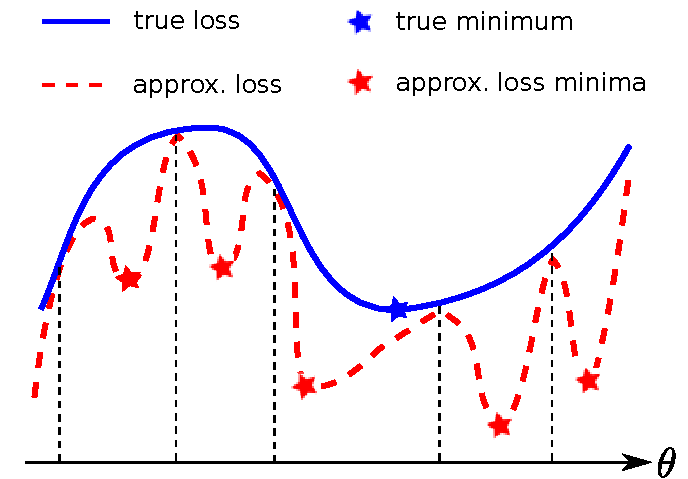
\includegraphics[width=0.45\linewidth]{figs/approx_loss.pdf}}
\hfill
\subfigure[approximate gradients \label{fig:approx_gradient}]{
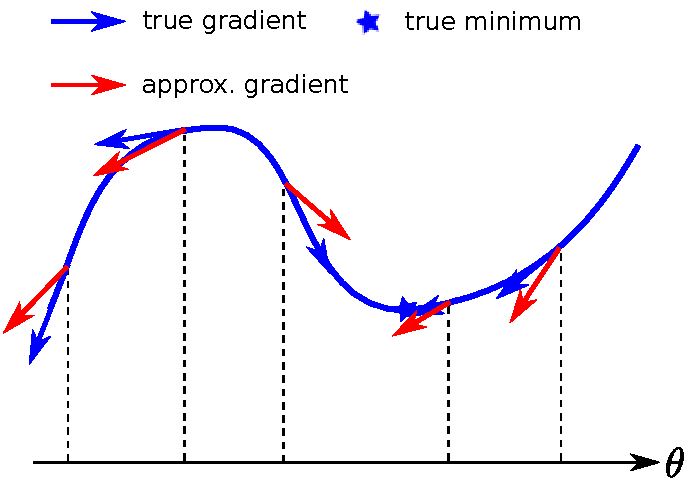
\includegraphics[width=0.45\linewidth]{figs/approx_gradient.pdf}}
\caption{A comparison between the two approximation schemes. Since in practice the optimiser only visits finite number of locations in the parameter space, it can lead to over-fitting if the neural network based functional approximator is not carefully regularised, and therefore the curvature information of the approximated loss can be very different from that of the original loss (shown in (a)). On the other hand, the gradient approximation scheme (b) can be more accurate since it only involves estimating the sensitivity of the loss function to the parameters in a local region.}
\label{fig:loss_grad_approx_compare}
\end{figure}

%Whilst prescribed probabilistic models can be learned by standard approximate maximum likelihood or Bayesian inference, implicit probabilistic models require more severe approximations due to the intractability of the model distribution. Many existing approaches first approximate the model distribution and/or optimisation objective functions, then learn the associated parameters using the defined approximations. For example, GANs use a discriminator which serves as a critic of the generative model, and let both networks play a minimax game until convergence. However, for finite number of data-points, there are infinite number of functions that could perfectly approximate the exact objective function evaluated at those observations, and for some of these approximating functions the gradient directions can be arbitrary far away from the exact ones. This is especially true when the approximated objective function is represented by neural network critics, where recent advances for stabilising GANs suggest restricting the representation power of the discriminator (e.g. see \citep{arjovsky:wgan2017}). There exist similar issues for variational methods as well, i.e.~proposing a lower-bound/upper-bound to the exact loss function. Similar to the variational lower-bound, these bounds are unlikely to be equally tight everywhere \citep{turner:two_problems2011}. It often biases the approximate posterior towards under-estimating uncertainty, and similarly for GANs the same problem exists as mode collapsing.

In the previous chapter a number of proposals for wild approximate inference are presented. Critically, we believe these techniques are extendable to learning implicit models, and in this chapter we explore the \emph{direct gradient approximation} idea as an alternative. A visualisation of the two approximation schemes is provided in Figure \ref{fig:loss_grad_approx_compare}. More specifically we focus on approximating the score function, in which an accurate approximation of it then allows the application of many well-studied algorithms, such as maximum likelihood, maximum entropy estimation, variational inference and gradient-based MCMC, to implicit models. Concretely, our contributions include:  
\begin{itemize}
\item the \emph{Stein gradient estimator}, a novel generalisation of the score matching estimator \citep{hyvarinen:score2005}, with both parametric and non-parametric versions;
\item a comparison of the proposed estimator with the score matching and the KDE plug-in estimators on performing gradient-free MCMC, meta-learning of approximate posterior samplers for Bayesian neural networks, and entropy based regularisation of GANs.
\end{itemize}

%In this paper we explore an alternative idea of training implicit models, which directly approximates the gradient of the implicit model distribution. More precisely we focus on approximating the score function $\nabla_{\x} \log q(\x)$ for some distribution $q$ to be learned. The score function is widely used in machine learning algorithms, e.g.~maximum likelihood, variational inference and gradient-based MCMC. Hence an accurate approximation to the score function would enable the application of these well-studied algorithms to implicit models. After reviewing recent advances in implicit models and gradient approximation techniques, we make the following contributions:  
%\begin{itemize}
%\item We propose the \emph{Stein gradient estimator} as a novel generalisation of the score matching estimator \citep{hyvarinen:score2005}, with both parametric and non-parametric versions presented;
%\item We compare the Stein estimator with the score matching estimator and the KDE plug-in estimator on three different tasks: gradient-free MCMC, entropy regularised GANs, and meta-learning of approximate posterior samplers for Bayesian neural networks.
%\end{itemize}

\section{Learning implicit probabilistic models}

Given a dataset $\mathcal{D}$ containing i.i.d.~samples we would like to learn a probabilistic model $p(\x)$ for the underlying data distribution $p_{\data}(\x)$. In the case of implicit models, $p(\x)$ is defined by a generative process. For example, to generate images, one might define a generative model $p(\x)$ that consists of sampling randomly a latent variable $\z \sim p_0(\z)$ and then defining $\x = \f_{\mparam}(\z)$. Here $\f$ is a function parametrised by $\mparam$, usually a deep neural network or a simulator. We assume $\f$ to be differentiable w.r.t.~$\mparam$. An extension to this scenario is presented by \emph{conditional} implicit models, where the addition of a supervision signal $\y$, such as an image label, allows us to define a conditional distribution $p(\x| \y)$ implicitly by the transformation $\x = \f_{\mparam}(\z, \y)$. A related methodology, \emph{wild approximate inference} (Chapter \ref{chap:wild}) assumes a tractable joint density $p(\x, \z)$, but uses implicit proposal distributions to approximate an intractable exact posterior $p(\z|\x)$. Here the approximate posterior $q(\z|\x)$ can likewise be represented by a deep neural network, but also by a truncated Markov chain, such as that given by Langevin dynamics with learnable step-size. 

%Given a dataset $\mathcal{D}$ containing i.i.d.~samples of the data distribution $p_{\data}(\x)$, we would like to learn it with a probabilistic model $p(\x)$. Implicit models usually define this distribution by describing a generative process. Taking image generation as an example, the generative model $p(\x)$ is defined by first sampling some random configuration of a latent variable $\z \sim p_0(\z)$, then transforming it into $\x = \f_{\mparam}(\z)$ with a function $\f$ parametrised by $\mparam$. In the rest of the paper we assume $\f$ is differentiable w.r.t.~$\mparam$. Such function can be represented by a deep neural network or a simulator. \emph{Conditional} implicit models have also been studied in the literature, for example, one can add in supervision signals $\y$, e.g.~labels of the image, and define $p(\x| \y)$ implicitly by the transformation $\x = \f_{\mparam}(\z, \y), \z \sim p_0(\z)$. On the other hand, \emph{wild variational inference} \citep{liu:two_wild2016, li:wild2016} assumes a tractable joint density $p(\x, \z)$ but proposes using implicit distributions to approximate the intractable exact posterior $p(\z|\x)$. Here the approximate posterior $q(\z|\x)$ can also be represented by a deep neural network, or a truncated Markov chain such as Langevin dynamics with learnable step-size. 

Whilst providing extreme flexibility and expressive power, the intractability of density evaluation also brings serious optimisation issues for implicit models. This is because many learning algorithms, e.g.~maximum likelihood estimation (MLE), rely on minimising a distance/divergence/discrepancy measure $\mathrm{D}[p || p_{\data}]$, which often requires evaluating the model density \citep[c.f.][]{ranganath:ovi2016, liu:two_wild2016}. Thus good approximations to the optimisation procedure are the key to learning implicit models that can describe complex data structure. In the context of GANs, the Jensen-Shannon divergence is approximated by a variational lower-bound represented by a discriminator \citep{barber:vim2003, goodfellow:gan2014}. 
%
Related work for wild variational inference \citep{li:wild2016, mescheder:avb2017, huszar:implicit2017, tran:implicit2017} uses a GAN-based technique to construct a density ratio estimator for $q / p_0$ \citep{sugiyama:ratio2009, sugiyama:ratio2012, uehara:gan2016, mohamed:gan2016} and then approximates the KL-divergence term in the variational lower-bound:
\begin{equation}
\mathcal{L}_{\text{VI}}(q) = \mathbb{E}_{q} \left[ \log p(\x | \z) \right] - \mathrm{KL}[q_{\vparam}(\z|\x) || p_0(\z)].
\end{equation} 
In addition, \cite{li:wild2016} and \cite{mescheder:avb2017} exploit the additive structure of the KL-divergence and suggest discriminating between $q$ and an auxiliary distribution that is close to $q$, making the density ratio estimation more accurate. Nevertheless all these algorithms involve a minimax optimisation, and the current practice of gradient-based optimisation is notoriously unstable. 

The stabilisation of GAN training is itself a recent trend of related research \citep[e.g.~see][]{salimans:training2016, arjovsky:wgan2017}. However, as the gradient-based optimisation only interacts with gradients, there is no need to use a discriminator if an accurate approximation to the intractable gradients could be obtained. As an example, consider a variational inference task with the approximate posterior defined as $\z \sim q_{\vparam}(\z | \x) \Leftrightarrow \bm{\epsilon} \sim \pi(\bm{\epsilon}), \z = \f_{\vparam}(\bm{\epsilon}, \x)$. Notice that the variational lower-bound can be rewritten as
\begin{equation}
\mathcal{L}_{\text{VI}}(q) = \mathbb{E}_{q} \left[ \log p(\x, \z) \right]  + \mathbb{H}[q_{\vparam}(\z | \x)],
\label{eq:vi_objective_entropy}
\end{equation}
the gradient of the variational parameters $\vparam$ can be computed by a sum of the path gradient of the first term (i.e.~$\mathbb{E}_{\pi} \left[ \nabla_{\f} \log p(\x, \f(\noise, \x))^{\text{T}} \nabla_{\vparam} \f(\noise, \x) \right] $) and the gradient of the entropy term $\nabla_{\vparam} \mathbb{H}[q(\z | \x)]$. Expanding the latter, we have 
%\begin{equation}
%-\nabla_{\vparam} \mathbb{H}[q(\z | \x)] = \mathbb{E}_{\pi} \left[ \nabla_{\f} \log q(\f(\noise, \x) | \x)^{\text{T}} \nabla_{\vparam} \f(\noise, \x)] \right] + \mathbb{E}_{q} \left[ \nabla_{\vparam} \log q_{\vparam}(\z | \x) \right],
%\label{eq:entropy_gradient}
%\end{equation}
\begin{equation}
\begin{aligned}
\nabla_{\vparam} \mathbb{H}[q_{\vparam}(\z | \x)] 
&= - \nabla_{\vparam} \mathbb{E}_{\pi(\bm{\epsilon})}[\log q_{\vparam}(\f_{\vparam}(\bm{\epsilon}, \x))] \\
&= - \mathbb{E}_{\pi(\bm{\epsilon})}[ \nabla_{\vparam} \log q_{\vparam}(\f_{\vparam}(\bm{\epsilon}, \x))] \\
&= - \mathbb{E}_{\pi(\bm{\epsilon})}[ \nabla_{\vparam} \log q_{\vparam}(\z | \x) |_{\z = \f_{\vparam}(\bm{\epsilon}, \x)} +  \nabla_{\vparam} \f_{\vparam}(\bm{\epsilon}, \x)  \nabla_{\f} \log q_{\vparam}(\f_{\vparam}(\bm{\epsilon}, \x) | \x) ] \\
&= - \mathbb{E}_{q_{\vparam}(\z | \x)} [ \nabla_{\vparam} \log q_{\vparam}(\z | \x)] - \mathbb{E}_{\pi(\bm{\epsilon})} [ \nabla_{\vparam} \f_{\vparam}(\bm{\epsilon}, \x) \nabla_{\f} \log q_{\vparam}(\f_{\vparam}(\bm{\epsilon}, \x) | \x)  ],
\end{aligned}
\label{eq:entropy_gradient}
\end{equation}
in which the first term in the last line is zero \citep{roeder:sticking2017}. As we typically assume the tractability of $\nabla_{\vparam} \f$, an accurate approximation to $\nabla_{\z} \log q(\z | \x)$ would remove the requirement of discriminators, speed-up the learning and obtain potentially a better model.
%
Many gradient approximation techniques exist \citep{stone:spline1985, fan:local_poly1996, zhou:spline2000, debrabanter:lpr2013}, and in particular, in the next section we will review kernel-based methods such as kernel density estimation \citep{singh:kernel_gradient1977} and score matching \citep{hyvarinen:score2005} in more detail, and motivate the main contribution of this chapter.


\section{Gradient approximation with the Stein gradient estimator}
\label{sec:gradient_approximation}

We propose the \emph{Stein gradient estimator} as a novel generalisation of the score matching gradient estimator. Before presenting it we first set-up the notation. Column vectors and matrices are boldfaced. The random variable under consideration is $\x \in \mathcal{X}$ with $\mathcal{X} = \mathbb{R}^{d \times 1}$ if not specifically mentioned. To avoid misleading notation we use the distribution $q(\x)$ to derive the gradient approximations for general cases. As Monte Carlo methods are heavily used for implicit models, in the rest of the paper we mainly consider approximating the gradient $\g(\x^k) :=\nabla_{\x^k} \log q(\x^k)$ for $\x^k \sim q(\x), k = 1, ..., K$. We use $x^i_j$ to denote the $j$th element of the $i$th sample $\x^i$. We also denote the matrix form of the collected gradients as
$\Grad := \left( \nabla_{\x^1} \log q(\x^1), \cdots, \nabla_{\x^K} \log q(\x^K) \right)^{\text{T}} \in \mathbb{R}^{K \times d}$, and its approximation $\hat{\Grad} := \left( \hat{g}(\x^1), \cdots, \hat{g}(\x^K) \right)^{\text{T}}$ with $\hat{g}(\x^k) = \nabla_{\x^k} \log \hat{q}(\x^k)$ for some $\hat{q}(\x)$.

\subsection{Stein gradient estimator: inverting Stein's identity}
We start from introducing \emph{Stein's identity} that was first developed for Gaussian random variables \citep{stein:stein_method1972, stein:stein_method_multi1981} then extended to general cases \citep{gorham:stein_method2015, liu:ksd2016}.
%
Let $\h: \mathbb{R}^{d \times 1} \rightarrow \mathbb{R}^{d' \times 1}$ be a differentiable multivariate test function which maps $\x$ to a column vector $\h(\x) = [h_1(\x), h_2(\x), ..., h_{d'}(\x)]^{\text{T}}$. We further assume the \emph{boundary condition} for $\h$: 
\begin{equation}
q(\x)\h(\x) |_{\partial \mathcal{X}} = \bm{0}, \text{ or } \lim_{\x \rightarrow \bm{\infty}} q(\x) \h(\x) = 0 \text{ if } \mathcal{X} = \mathbb{R}^d.
\label{eq:boundary_condition}
\end{equation}
This condition holds for almost any test function if $q$ has sufficiently fast-decaying tails (e.g.~Gaussian tails).
%
Now we introduce Stein's identity \citep{stein:stein_method_multi1981, gorham:stein_method2015, liu:ksd2016}
\begin{equation}
\mathbb{E}_{q}[\h(\x) \nabla_{\x} \log q(\x)^{\text{T}} + \nabla_{\x} \h(\x) ] = \bm{0}, 
\label{eq:stein_identity_multi}
\end{equation}
in which the gradient matrix term
$
\nabla_{\x} \h(\x) = \left( \nabla_{\x} h_1(\x), \cdots, \nabla_{\x} h_{d'}(\x) \right)^{\text{T}} \in \mathbb{R}^{d' \times d}.
$
This identity can be proved using \emph{integration by parts}: for the $i$th row of the matrix $\h(\x) \nabla_{\x} \log q(\x)^{\text{T}}$, we have
\begin{equation}
\begin{aligned}
\mathbb{E}_{q}[ h_i(\x) \nabla_{\x} \log q(\x)^{\text{T}}]
&= \int h_i(\x) \nabla_{\x} q(\x)^{\text{T}} d \x \\
&= q(\x)h_i(\x) |_{\partial \mathcal{X}} - \int q(\x)  \nabla_{\x} h_i(\x)^{\text{T}} d \x \\
&= - \mathbb{E}_{q} [\nabla_{\x} h_i(\x)^{\text{T}}].
\end{aligned}
\label{eq:integration_by_parts}
\end{equation}
Observing that the gradient term $\nabla_{\x} \log q(\x)$ of interest appears in Stein's identity (\ref{eq:stein_identity_multi}), we propose the \emph{Stein gradient estimator} by inverting Stein's identity. As the expectation in (\ref{eq:stein_identity_multi}) is intractable, we further approximate the above with Monte Carlo (MC):
\begin{equation}
\frac{1}{K} \sum_{k=1}^K -\h(\x^k) \nabla_{\x^k} \log q(\x^k)^{\text{T}} + \text{err} = \frac{1}{K} \sum_{k=1}^K \nabla_{\x^k} \h(\x^k), \quad \x^k \sim q(\x^k),
\label{eq:stein_multi_mc}
\end{equation}
with $\text{err} \in \mathbb{R}^{d' \times d}$ the random error due to MC approximation, which has mean $\bm{0}$ and vanishes as $K \rightarrow +\infty$. Now by temporarily denoting
$$
\Hmatrix = \left( \h(\x^1), \cdots , \h(\x^K) \right) \in \mathbb{R}^{d' \times K}, \quad
\hgrad = \frac{1}{K} \sum_{k=1}^K \nabla_{\x^k} \h(\x^k) \in \mathbb{R}^{d' \times d},
$$
equation (\ref{eq:stein_multi_mc}) can be rewritten as
$$-\frac{1}{K} \Hmatrix \Grad + \text{err} = \hgrad.$$
Thus we consider a ridge regression method (i.e. adding an $\ell_2$ regulariser) to estimate $\Grad$:
\begin{equation}
\hat{\Grad}_V^{\text{Stein}} := \argmin_{\hat{\Grad} \in \mathbb{R}^{K \times d} } || \hgrad + \frac{1}{K} \Hmatrix \hat{\Grad} ||_{F}^2 + \frac{\eta}{K^2} || \hat{\Grad} ||_{F}^2,
\label{eq:stein_objective}
\end{equation}
with $|| \cdot ||_{F}$ the Frobenius norm of a matrix and $\eta \geq 0$. Simple calculation shows that
\begin{equation}
\hat{\Grad}_V^{\text{Stein}} = -( \K + \eta \bm{I} )^{-1} \langle \nabla, \K \rangle,
\label{eq:stein_estimator}
\end{equation}
where 
$$\K := \Hmatrix^{\text{T}} \Hmatrix, \quad \K_{ij} = \mathcal{K}(\x^i, \x^j) := \h(\x^i)^{\text{T}} \h(\x^j),$$
$$\langle \nabla, \K \rangle := K \Hmatrix^{\text{T}} \hgrad, \quad \langle \nabla, \K \rangle_{ij} = \sum_{k=1}^{K} \nabla_{x^k_j} \mathcal{K}(\x^i, \x^k).$$
%
One can show that the RBF kernel satisfies Stein's identity \citep{liu:ksd2016}. In this case $\h(\x) = \mathcal{K}(\x, \cdot), d' = +\infty$ and by the reproducing kernel property  \citep{berlinet:rkhs2011},
$\h(\x)^{\text{T}} \h(\x') = \langle \mathcal{K}(\x, \cdot), \mathcal{K}(\x', \cdot) \rangle_{\mathcal{H}} = \mathcal{K}(\x, \x') .$

\subsection{Stein gradient estimator minimises the kernelised Stein discrepancy}
In this section we derive the Stein gradient estimator again, but from a divergence/discrepancy minimisation perspective. 
%
Stein's method also provides a tool for checking if two distributions $q(\x)$ and $\hat{q}(\x)$ are identical. If the test function set $\mathcal{H}$ (containing one-dimensional test functions $h \in \mathcal{H}$) is sufficiently rich, then one can define a Stein discrepancy measure (equipped with norm $|| \cdot ||$) by
\begin{equation}
\mathcal{S}(q, \hat{q}) := \sup_{\h \in \mathcal{H}} || \mathbb{E}_{q} \left[ \nabla_{\x} \log \hat{q}(\x) h(\x) + \nabla_{\x} h(\x) \right] ||,
\label{eq:stein_discrepancy}
\end{equation}
see \cite{gorham:stein_method2015} for an example derivation. The definition can be generalised to multi-dimension test functions $\h(\x)$, and in particular, when $\mathcal{H}$ is defined as a unit ball in an RKHS induced by a kernel $\mathcal{K}(\x, \cdot)$ and $|| \cdot ||$ is the $\ell_2$ norm, \cite{liu:ksd2016} and \cite{chwialkowski:ksd2016} showed that the supremum in (\ref{eq:stein_discrepancy}) can be analytically obtained as (recall $\g(\x) = \nabla_{\x} \log q(\x), \hat{\g}(\x) = \nabla_{\x} \log \hat{q}(\x)$): 
\begin{equation}
\mathcal{S}^2(q, \hat{q}) = \mathbb{E}_{\x, \x' \sim q} \left[ (\hat{\g}(\x) - \g(\x) )^{\text{T}} \mathcal{K}(\x, \x') (\hat{\g}(\x') - \g(\x') ) \right],
\label{eq:ksd}
\end{equation}
which is also named the \emph{kernelised Stein discrepancy} (KSD). \cite{chwialkowski:ksd2016} showed that for $C_0$-universal kernels satisfying the boundary condition, KSD is indeed a discrepancy measure: $\mathcal{S}^2(q, \hat{q}) = 0 \Leftrightarrow q = \hat{q}$.  \cite{gorham:ksd2017} further characterised the power of KSD on detecting non-convergence cases. Furthermore, if the kernel is twice differentiable, then using the same technique as to derive (\ref{eq:score_matching_objective}) one can compute KSD by  (with $\mathcal{K}_{\x \x'}$ shorthand for $\mathcal{K}(\x, \x')$):
\begin{equation}
\mathcal{S}^2(q, \hat{q}) = \mathbb{E}_{\x, \x' \sim q} \left[ \hat{\g}(\x)^{\text{T}} \mathcal{K}_{\x \x'} \hat{\g}(\x') + \hat{\g}(\x)^{\text{T}} \nabla_{\x'} \mathcal{K}_{\x \x'} + \nabla_{\x} \mathcal{K}_{\x \x'}^{\text{T}} \hat{\g}(\x') + \text{Tr}(\nabla_{\x, \x'} \mathcal{K}_{\x \x'} )\right].
\label{eq:ksd_transformed}
\end{equation}
In practice KSD is estimated with samples $\{ \x^k \}_{k=1}^K \sim q$, and simple derivations show that the V-statistic of KSD can be reformulated as $\mathcal{S}_{V}^2(q, \hat{q}) = \frac{1}{K^2} \text{Tr} (\hat{\Grad}^{\text{T}} \K \hat{\Grad} + 2 \hat{\Grad}^{\text{T}} \langle \nabla, \K \rangle) + C$.
%
Thus the $l_2$ error in (\ref{eq:stein_objective}) is equivalent to the V-statistic of KSD if $\h(\x) = \mathcal{K}(\x, \cdot)$, and we have the following:
\begin{theorem}
$\hat{\Grad}_V^{\text{\emph{Stein}}}$ is the solution of the following KSD V-statistic minimisation problem
\begin{equation}
\hat{\Grad}_V^{\text{\emph{Stein}}} = \argmin_{\hat{\Grad} \in \mathbb{R}^{K \times d}} \quad \mathcal{S}_{V}^2(q, \hat{q}) + \frac{\eta}{ K^2} ||\hat{\Grad}||_F^2 .
\end{equation}
\label{thm:stein_ksd}
\vspace{-0.2in}
\end{theorem}
%
One can also minimise the U-statistic of KSD to obtain gradient approximations, and a full derivation of which, including the optimal solution, can be found in Appendix \ref{sec:appendix_stein}. In experiments we use V-statistic solutions and leave comparisons between these methods to future work.

\subsection{Comparisons to existing kernel-based gradient estimators}
There exist other gradient estimators that do not require explicit evaluations of $\nabla_{\x} \log q(\x)$, e.g.~the denoising auto-encoder (DAE) \citep{vincent:denoising2008, vincent:denoising2011, alain:denoising2014} which, with infinitesimal noise, also provides an estimate of $\nabla_{\x} \log q(\x)$ at convergence. However, applying such gradient estimators result in a double-loop optimisation procedure since the gradient approximation is repeatedly required for fitting implicit distributions, which can be significantly slower than the proposed approach. Therefore we focus on ``quick and dirty'' approximations and only include comparisons to kernel-based gradient estimators in the following.

\subsubsection{KDE gradient estimator: plug-in estimator with density estimation}
A naive approach for gradient approximation would first estimate the intractable density $\hat{q}(\x) \approx q(\x)$ (up to a constant), then approximate the exact gradient by $\nabla_{\x} \log \hat{q}(\x) \approx \nabla_{\x} \log q(\x)$. Specifically, \cite{singh:kernel_gradient1977} considered kernel density estimation (KDE) 
$\hat{q}(\x) = \frac{1}{K} \sum_{k=1}^K \mathcal{K}(\x, \x^k) \times C.$, then differentiated through the KDE estimate to obtain the gradient estimator:
\begin{equation}
\hat{\Grad}^{\text{KDE}}_{ij} = \sum_{k=1}^K \nabla_{x^i_j} \mathcal{K}(\x^i, \x^k) / \sum_{k=1}^K \mathcal{K}(\x^i, \x^k).
\label{eq:kde_estimator}
\end{equation}
%
Interestingly for translation invariant kernels $\mathcal{K}(\x, \x') = \mathcal{K}(\x - \x')$ the \emph{KDE gradient estimator} (\ref{eq:kde_estimator}) can be rewritten as $\hat{\Grad}^{\text{KDE}} = -\text{diag}\left( \K \bm{1} \right)^{-1} \langle \nabla, \K \rangle.$
Inspecting and comparing it with the Stein gradient estimator (\ref{eq:stein_estimator}), one might notice that the Stein method uses the full kernel matrix as the pre-conditioner, while the KDE method computes an averaged ``kernel similarity'' for the denominator. We conjecture that this difference is key to the superior performance of the Stein gradient estimator when compared to the KDE gradient estimator (see later experiments). The KDE method only collects the similarity information between $\x^k$ and other samples $\x^j$ to form an estimate of $\nabla_{\x^k} \log q(\x^k)$, whereas for the Stein gradient estimator, the kernel similarity between $\x^i$ and $\x^j$ for all $i, j \neq k$ are also incorporated. Thus it is reasonable to conjecture that the Stein method can be more sample efficient, which also implies higher accuracy when the same number of samples are collected.

\subsubsection{Score matching gradient estimator: minimising MSE}
\label{sec:score_matching}
The KDE gradient estimator performs indirect approximation of the gradient via density estimation, which can be inaccurate. An alternative approach directly approximates the gradient $\nabla_{\x} \log q(\x)$ by minimising the expected $\ell_2$ error w.r.t.~the approximation $\hat{\g}(\x) = \left(\hat{g}_1(\x), \cdots, \hat{g}_d(\x) \right)^{\text{T}}$:
\begin{equation}
\mathcal{F}(\hat{\g}) := \mathbb{E}_{q} \left[ || \hat{\g}(\x) - \nabla_{\x} \log q(\x) ||_2^2 \right].
\label{eq:fisher_divergence}
\end{equation}
It has been shown in \cite{hyvarinen:score2005} that this objective can be reformulated as
\begin{equation}
\mathcal{F}(\hat{\g}) = \mathbb{E}_{q} \left[ || \hat{\g}(\x) ||_2^2 + 2 \langle \nabla, \hat{\g}(\x) \rangle \right] + C, \quad \langle \nabla, \hat{\g}(\x) \rangle = \sum_{j=1}^d \nabla_{x_j} \hat{g}_j(\x).
\label{eq:score_matching_objective}
\end{equation}
The key insight here is again the usage of integration by parts: after expanding the $\ell_2$ loss objective, the cross term can be rewritten as
$\mathbb{E}_q \left[ \hat{\g}(\x)^{\text{T}} \nabla_{\x} \log q(\x) \right] = -\mathbb{E}_q \left[ \langle \nabla, \hat{\g}(\x) \rangle \right],$
if assuming the boundary condition (\ref{eq:boundary_condition}) for $\hat{\g}$ (see (\ref{eq:integration_by_parts})). 
%
The optimum of (\ref{eq:score_matching_objective}) is referred as the \emph{score matching gradient estimator}. 
%
The $\ell_2$ objective (\ref{eq:fisher_divergence}) is also called \emph{Fisher divergence} \citep{johnson:itbook2004} which is a special case of KSD (\ref{eq:ksd}) by selecting $\mathcal{K}(\x, \x') = \delta_{\x = \x'}$. Thus the Stein gradient estimator can be viewed as a generalisation of the score matching estimator. 
%
%A slightly different approach \citep{sasaki:gradient2015} proposes an estimator for $\nabla_{\x} q(\x)$, by minimising the $l_2$ error $\int (\hat{g}_j(\x) - \nabla_{x_j} q(\x))^2 d\x$ and removing explicit calculations of $\nabla_{\x} q(\x)$ in an analogous way as to derive (\ref{eq:score_matching_objective}). 

The comparison between the two estimators is more complicated. Certainly by the Cauchy-Schwarz inequality the Fisher divergence is stronger than KSD in terms of detecting convergence \citep{liu:ksd2016}. However it is difficult to perform direct gradient estimation by minimising the Fisher divergence, since (i) the Dirac kernel is non-differentiable so that it is impossible to rewrite the divergence in a similar form to (\ref{eq:ksd_transformed}), and (ii) the transformation to (\ref{eq:score_matching_objective}) involves computing $\nabla_{\x} \hat{\g}(\x)$. So one needs to propose a \emph{parametric} approximation to $\Grad$ and then optimise the associated parameters accordingly, and indeed \cite{sasaki:gradient2014} and \cite{strathmann:kmc2015} derived a parametric solution by first approximating the log density up to a constant as
$\log \hat{q}(\x) := \sum_{k=1}^K a_k \mathcal{K}(\x, \x^k) + C$,
then minimising (\ref{eq:score_matching_objective}) to obtain the coefficients $\hat{a}^{\text{score}}_k$ and constructing the gradient estimator as
\begin{equation}
\hat{\Grad}^{\text{score}}_{i\cdot} = \sum_{k=1}^{K} \hat{a}^{\text{score}}_k \nabla_{\x^i} \mathcal{K}(\x^i, \x^k).
\label{eq:grad_parametric_estimator}
\end{equation}
%
Therefore the usage of parametric estimation can potentially remove the advantage of using a stronger divergence. Conversely, the proposed Stein gradient estimator (\ref{eq:stein_estimator}) is \emph{non-parametric} in that it directly optimises over functions evaluated at locations $\{ \x_k \}_{k=1}^K$. 
%
This brings in two key advantages over the score matching gradient estimator: (i) it removes the \emph{approximation error} due to the use of restricted family of parametric approximations and thus can be potentially more accurate; (ii) it has a much simpler and \emph{ubiquitous} form that applies to \emph{any kernel satisfying the boundary condition}, whereas the score matching estimator requires tedious derivations for different kernels repeatedly (see Appendix \ref{sec:appendix_stein}). 

In terms of computation speed, since in most of the cases the computation of the score matching gradient estimator also involves kernel matrix inversions, both estimators are of the same order of complexity, which is $\mathcal{O}(K^3 + K^2 d)$ (kernel matrix computation plus inversion). Low-rank approximations such as the Nystr\"om method \citep{smola:sparse2000, williams:kernel2001} can enable speed-up, but this is not investigated in the paper. Again we note here that kernel-based gradient estimators can still be faster than e.g.~the DAE estimator since no double-loop optimisation is required. Certainly it is possible to apply early-stopping for the inner-loop DAE fitting. However the resulting gradient approximation might be very poor, which leads to unstable training and poorly fitted implicit distributions.

\vspace{1em}
\begin{tcolorbox}
\textbf{Remark} (score matching methods)\textbf{.}
As a side note, score matching can also be used to learn the parameters of an unnormalised density. In this case the target distribution $q$ would be the data distribution and $\hat{q}$ is often a Boltzmann distribution with intractable partition function. As a parameter estimation technique, score matching is also related to contrastive divergence \citep{hinton:cd2002}, pseudo likelihood estimation \citep{hyvarinen:pseudolikelihood2006}, and denoising auto-encoders \citep{vincent:denoising2011}. Generalisations of score matching methods are also presented in \citep{lyu:score2009, marlin:rbm2010}.
\end{tcolorbox}

\subsection{Adding predictive power}
\label{sec:predictive_estimator}
Though providing potentially more accurate approximations, the non-parametric estimator (\ref{eq:stein_estimator}) has no predictive power as described so far. Crucially, many tasks in machine learning require predicting gradient functions at samples drawn from distributions other than $q$, for example, in MLE $q(\x)$ corresponds to the model distribution which is learned using samples from the data distribution instead. To address this issue, we derive two \emph{predictive} estimators, one generalised from the non-parametric estimator and the other minimises KSD using parametric approximations.

\paragraph{Predictions using the non-parametric estimator.}

Let us consider an unseen datum $\y$. If $\y$ is sampled from $q$, then one can also apply the non-parametric estimator (\ref{eq:stein_estimator}) for gradient approximation, given the observed data $\X = \{\x^1, ..., \x^K \} \sim q$. Concretely, if writing $\hat{\g}(\y) \approx \nabla_{\y} \log q(\y) \in \mathbb{R}^{d \times 1}$ then the non-parametric Stein gradient estimator computed on $\X \cup \{\y\}$ is
\begin{equation*}
\begin{bmatrix}
\hat{\g}(\y)^{\text{T}} \\
\hat{\Grad}
\end{bmatrix}
= -( \K^* + \eta \bm{I} )^{-1} 
\begin{bmatrix}
\nabla_{\y} \mathcal{K}(\y, \y) + \sum_{k=1}^{K} \nabla_{\x^k} \mathcal{K}(\y, \x^k) \\
\langle \nabla, \K \rangle + \nabla_{\y} \mathcal{K}(\cdot, \y)
\end{bmatrix}
, \quad 
\K^* = \begin{bmatrix}
    \K_{\y \y}       & \K_{\y\X} \\
    \K_{\X \y}       & \K
\end{bmatrix},
\end{equation*}
with $\nabla_{\y} \mathcal{K}(\cdot, \y)$ denoting a $K \times d$ matrix with rows $\nabla_{\y} \mathcal{K}(\x^k, \y)$, and $\nabla_{\y} \mathcal{K}(\y, \y)$ only differentiates through the second argument. Thus by simple matrix calculations, we have:
\begin{equation}
\begin{aligned}
\nabla_{\y} \log q(\y)^{\text{T}} \approx& -\left(\K_{\y\y} + \eta - \K_{\y\X} (\K + \eta \mathbf{I})^{-1} \K_{\X\y} \right)^{-1} \\&\left( \nabla_{\y} \mathcal{K}(\y, \y) + \sum_{k=1}^{K} \nabla_{\x^k} \mathcal{K}(\y, \x^k) + \K_{\y\X} \hat{\Grad}_{V}^{\text{Stein}} - \K_{\y\X} (\K + \eta \mathbf{I})^{-1} \nabla_{\y} \mathcal{K}(\cdot, \y) \right).
\end{aligned}
\label{eq:stein_estimator_predict}
\end{equation}
For translation invariant kernels, typically $\nabla_{\y} \mathcal{K}(\y, \y) = \bm{0}$, and more conveniently, 
$$ \nabla_{\x^k} \mathcal{K}(\y, \x^k) = \nabla_{\x^k} (\x^k - \y) \nabla_{(\x^k - \y)} \mathcal{K}(\x^k - \y) = - \nabla_{\y} \mathcal{K}(\x^k, \y).$$
Thus equation (\ref{eq:stein_estimator_predict}) can be further simplified to (with column vector $\bm{1} \in \mathbb{R}^{K \times 1}$)
\begin{equation}
\begin{aligned}
\nabla_{\y} \log q(\y)^{\text{T}} \approx& -\left(\K_{\y\y} + \eta - \K_{\y\X} (\K + \eta \mathbf{I})^{-1} \K_{\X\y} \right)^{-1} \\&\left( \K_{\y\X} \hat{\Grad}_{V}^{\text{Stein}} - \left( \K_{\y\X} (\K + \eta \mathbf{I})^{-1} + \bm{1}^{\text{T}} \right) \nabla_{\y} \mathcal{K}(\cdot, \y) \right).
\end{aligned}
\label{eq:stein_estimator_predict_simplified}
\end{equation}
%
In practice one would store the computed gradient $\hat{\Grad}_{V}^{\text{Stein}}$, the kernel matrix inverse $(\K + \eta \mathbf{I})^{-1}$ and $\eta$ as the ``parameters'' of the predictive estimator.
%
For a new observation $\y \sim p$ in general, one can ``pretend'' $\y$ is a sample from $q$ and apply the above estimator as well. The approximation quality depends on the similarity between $q$ and $p$, and we conjecture here that this similarity measure, if can be described, is closely related to the KSD.
 
\paragraph{Fitting a parametric estimator using KSD.}
The non-parametric predictive estimator could be computationally demanding. Setting aside the cost of fitting the ``parameters'', in prediction the time complexity for the non-parametric estimator is $\mathcal{O}(K^2 + Kd)$. Also storing the ``parameters'' needs $\mathcal{O}(Kd)$ memory for $\hat{\Grad}_{V}^{\text{Stein}}$ and $(\K + \eta \mathbf{I})^{-1}$. These costs make the non-parametric estimator undesirable for high-dimensional data, since in order to obtain accurate predictions it often requires $K$ scaling with $d$ as well. To address this, one can also minimise the KSD using parametric approximations, in a similar way as to derive the score matching estimator in Section \ref{sec:score_matching}. 
%
More precisely, we define a parametric approximation in a similar fashion as (\ref{eq:grad_parametric_estimator}), and in Appendix \ref{sec:appendix_stein} we show that if the RBF kernel is used for both the KSD and the parametric approximation, then the linear coefficients $\bm{a} = (a_1, ..., a_K)^{\text{T}}$ can be calculated analytically: $\hat{\bm{a}}_{V}^{\text{Stein}} = (\bm{\Lambda} + \eta \mathbf{I})^{-1} \bm{b}$, where
\begin{equation}
\begin{aligned}
\bm{\Lambda} =& \mathbb{X} \odot (\K \K \K) + \K (\K \odot \mathbb{X}) \K - ((\K\K) \odot \mathbb{X}) \K - \K ((\K\K) \odot \mathbb{X}), \\
\bm{b} =& ( \K \text{diag}(\mathbb{X}) \K + (\K \K) \odot \mathbb{X} - \K (\K \odot \mathbb{X}) - (\K \odot \mathbb{X}) \K ) \bm{1},
\end{aligned}
\end{equation}
%
with $\odot$ denoting element-wise product, and $\mathbb{X}$ denoting the ``gram matrix'' that has elements $\mathbb{X}_{ij} = (\x^i)^{\text{T}} \x^j$. Then for an unseen observation $\y \sim p$ the gradient approximation returns $\nabla_{\y} \log q(\y) \approx (\hat{\bm{a}}^{\text{Stein}}_{V})^{\text{T}} \nabla_{\y} \mathcal{K}(\cdot, \y)$. In this case one only maintains the linear coefficients $\hat{\bm{a}}^{\text{Stein}}_{V}$ and computes a linear combination in prediction, which takes $\mathcal{O}(K)$ memory and $\mathcal{O}(Kd)$ time and therefore is computationally cheaper than the non-parametric prediction model (\ref{eq:stein_estimator_predict}).



\section{Applications}
We present some case studies that apply the gradient estimators to implicit models. Detailed settings (architecture, learning rate, etc.) are presented in Appendix \ref{sec:appendix_stein}. Implementation is released at \url{https://github.com/YingzhenLi/SteinGrad}.

\subsection{Synthetic example: Hamiltonian flow with approximate gradients}
We first consider a simple synthetic example to demonstrate the accuracy of the proposed gradient estimator. More precisely we consider the kernel induced Hamiltonian flow (\emph{not} an exact sampler) \citep{strathmann:kmc2015} on a 2-dimensional banana-shaped object: $\x \sim \mathcal{B}(\x; b=0.03, v=100) \Leftrightarrow  x_1 \sim \mathcal{N}(x_1; 0, v), x_2 = \epsilon + b(x_1^2 - v), \epsilon \sim \mathcal{N}(\epsilon; 0, 1)$. The approximate Hamiltonian flow is constructed using the same operator as in Hamiltonian Monte Carlo (HMC) \citep{duane:hmc1987, neal:mcmc2011}, except that the exact score function $\nabla_{\x} \log \mathcal{B}(\x)$ is replaced by the approximate gradients. We still use the exact target density to compute the rejection step as we mainly focus on testing the accuracy of the gradient estimators. We test both versions of the predictive Stein gradient estimator (see Section \ref{sec:predictive_estimator}) since we require the particles of parallel chains to be independent with each other. 
%
We fit the gradient estimators on $K=200$ training datapoints from the target density. The bandwidth of the RBF kernel is computed by the median heuristic and scaled up by a scalar between $[1, 5]$. All three methods are simulated for $T=2,000$ iterations, they share the same initial locations that are constructed by target distribution samples plus Gaussian noises of standard deviation 2.0, and the results are averaged over 200 parallel chains. 

We visualise the samples and some MCMC statistics in Figure \ref{fig:banana_example}. 
%
In general all the resulting Hamiltonian flows
are HMC-like, which give us the confidence that the gradient estimators extrapolate reasonably well at unseen locations that are close to the training data. However all of these methods have trouble exploring the extremes, because at those locations there are very few or even no training data-points. Indeed we found it necessary to use large (but not too large) bandwidths, in order to both allow exploration of those extremes, and ensure that the corresponding test function is not too smooth. In terms of quantitative metrics, the acceptance rates are reasonably high for all the gradient estimators, and the KSD estimates (across chains) as a measure of sample quality are also close to that computed on HMC samples. The returned estimates of $\mathbb{E}[x_1]$ are close to zero which is the ground true value. We found that the non-parametric Stein gradient estimator is more sensitive to hyper-parameters of the dynamics, e.g.~the stepsize of each HMC step.
%
We believe a careful selection of the kernel (e.g.~those with long tails) and a better search
for the hyper-parameters (for both the kernel and the dynamics) can further improve the
sample quality and the chain mixing time, but this is not investigated here.

\begin{figure}[t]
\vspace{-0.15in}
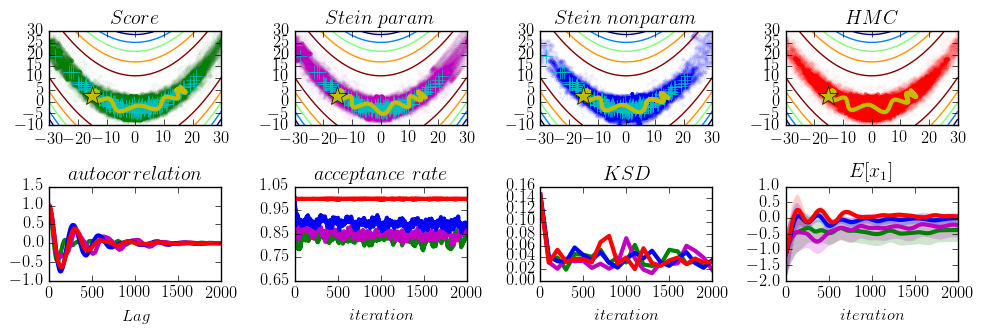
\includegraphics[width=1.0\linewidth]{figs/banana.png}
\vspace{-0.2in}
\caption{Kernel induced Hamiltonian flow compared with HMC. Top: samples generated from the dynamics, training data (in cyan), an the trajectory of a particle for $T=1$ to $200$ starting at the star location (in yellow). Bottom: statistics computed during simulations. See main text for details.}
\vspace{-0.1in}
\label{fig:banana_example}
\end{figure}

\subsection{Meta-learning of approximate posterior samplers for Bayesian NNs}
\label{sec:chap6_meta}
%
One of the recent focuses on meta-learning has been on learning optimisers for training deep neural networks, e.g.~see \cite{andrychowicz:gradient2016, li:optimize2016}. Could analogous goals be achieved for approximate inference? In this section we attempt to learn an approximate posterior sampler for Bayesian neural networks (Bayesian NNs, BNNs) that generalises to \emph{unseen} datasets and architectures, and we refer to Section \ref{sec:chap5_wild_applications} for a motivation of this approach. 

In a nutshell, we consider a binary classification task: $p(y = 1|\x, \mparam) = \text{sigmoid}(\text{NN}_{\mparam}(\x))$, $p_0(\mparam) = \mathcal{N}(\mparam; \bm{0}, \mathbf{I})$. After observing the training data $\data = \{(\x_n, y_n)\}_{n=1}^N$, we first obtain the approximate posterior $q_{\vparam}(\mparam) \approx p(\mparam | \data) \propto p_0(\mparam) \prod_{n=1}^N p(y_n | \x_n, \mparam)$, then approximate the predictive distribution for a new observation as $ p(y^*=1|\x^*, \data) \approx \frac{1}{K} \sum_{k=1}^K p(y^*=1|\x^*, \mparam^k), \mparam^k \sim q_{\vparam}(\mparam). $ 
%
In this task we define an implicit approximate posterior distribution $q_{\vparam}(\mparam)$ as the following \emph{stochastic} RNN $\mparam_{t+1} = \f(\mparam_t, \nabla_t, \bm{\epsilon}_t)$: given the current location $\mparam_t$ and the mini-batch data $\{ (\x_m, y_m) \}_{m=1}^M$, the update for the next step is
\begin{equation}
\begin{aligned}
\mparam_{t+1} &= \mparam_{t} + \zeta \Delta_{\vparam}(\mparam_t, \nabla_t) + \bm{\sigma}_{\vparam}(\mparam_t, \nabla_t) \odot \bm{\epsilon}_t, \quad \bm{\epsilon}_t \sim  \mathcal{N}(\bm{\epsilon}; \bm{0}, \mathbf{I}),\\
\nabla_t &= \nabla_{\mparam_t} \left[ \frac{N}{M} \sum_{m=1}^M \log p(y_m|\x_m, \mparam_t) + \log p_0(\mparam_t) \right] .
\end{aligned}
\end{equation}
The coordinates of the noise standard deviation $\bm{\sigma}_{\vparam}(\mparam_t, \nabla_t)$ and the moving direction $\Delta_{\vparam}(\mparam_t, \nabla_t)$ are parametrised by a \emph{coordinate-wise} neural network, i.e.~
$$\bm{\sigma}_{\vparam}(\mparam_t, \nabla_t) = [\bm{\sigma}_{\vparam}(\mparam_t(1), \nabla_t(1)), ..., \bm{\sigma}_{\vparam}(\mparam_t(d), \nabla_t(d)) ]^{\text{T}}$$
with $\mparam_t(i)$ denoting the $i^{\text{th}}$ dimension of vector $\mparam_t$ (similarly for $\nabla_t(i)$ and $\Delta_{\vparam}(\mparam_t, \nabla_t)$).
%
If properly trained, this neural network will learn the best combination of the current location and gradient information, and produce approximate posterior samples efficiently on different probabilistic modelling tasks.

We propose using the variational inference objective (\ref{eq:vi_objective_entropy}) computed on the samples $\{ \mparam_t^k \}$ to learn the variational parameters $\vparam$. 
%
More specifically, we simulate the approximate sampler for $T = 10$ transitions and sum over the variational lower-bounds computed on the samples of every step. This gives the maximisation objective
$$\mathcal{L}(\vparam) = \sum_{t=1}^T \mathcal{L}_{\text{VI}}(q_t),$$
with $q_t(\mparam)$ as the marginal distribution of $\mparam_t$ (therefore depends on $\vparam$). In practice the variational lower-bound $\mathcal{L}_{\text{VI}}(q_t)$ is further approximated by Monte Carlo and data sub-sampling:
$$ \mathcal{L}_{\text{VI}}(q_t) \approx \frac{N}{K M} \sum_{m = 1}^M \sum_{k=1}^K \log p(y_m|\x_m, \mparam_t^k) + \log p_0(\mparam_t^k) - \log q_t(\mparam_t^k).$$
%
Since in this case the gradient of the log joint distribution can be computed analytically, we only approximate the gradient of the entropy term $\mathbb{H}[q]$ as in (\ref{eq:entropy_gradient}), with the exact score function replaced by the presented gradient estimators. 

\begin{figure}[t]
\subfigure[SGLD]{
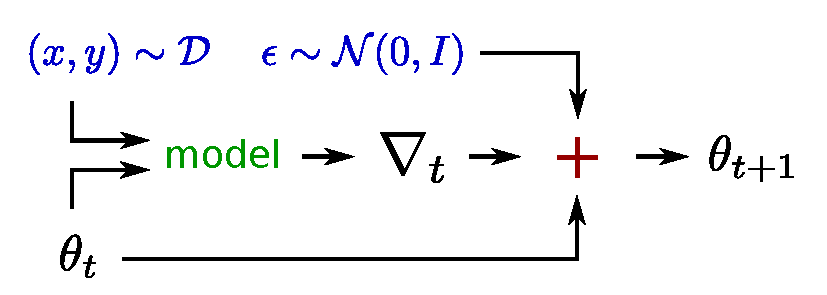
\includegraphics[width=0.45\linewidth]{figs/sgld_sampler.pdf}}
\hfill
\subfigure[NN-based approx.~sampler]{
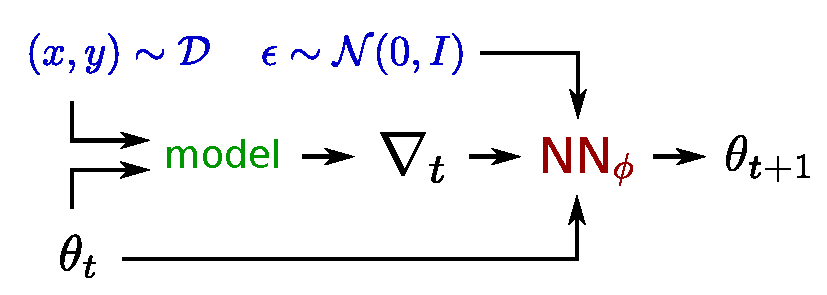
\includegraphics[width=0.45\linewidth]{figs/nn_sampler.pdf}}
\caption{Comparing the computation graphs of the two samplers. SGLD can be viewed as stochastic gradient descent plus properly scaled Gaussian noise. Instead of using the ``plus'' operation, the NN-based sampler combine the three inputs with a neural network, and the parameters $\vparam$ are then trained by the method described in the main text.}
\label{fig:sgld_nn_sampler_compare}
\end{figure}

We briefly describe the test protocol. We take from the UCI repository \citep{Lichman:uci_data2013} six binary classification datasets (australian, breast, crabs, ionosphere, pima, sonar), train an approximate sampler on crabs with a small neural network that has one 20-unit hidden layer with \emph{ReLU} activation, and generalise to the remaining datasets with a bigger network that has 50 hidden units and uses \emph{sigmoid} activation. We use ionosphere as the validation set to tune $\zeta$. The remaining 4 datasets are further split into 40\% training subset for simulating samples from the approximate sampler, and 60\% test subsets for evaluating the sampler's performance.
%
Besides the gradient estimators we also compare with two baselines: an approximate posterior sampler trained by maximum a posteriori (MAP), and stochastic gradient Langevin dynamics (SGLD) \citep{welling:sgld2011} evaluated on the test datasets directly. A comparison between SGLD and the proposed neural network based approximate sampler is visualised in Figure \ref{fig:sgld_nn_sampler_compare}. 

For architecture details, we use a one hidden layer neural network with 20 hidden units to compute the noise standard deviation $\bm{\sigma}_{\vparam}(\mparam_t, \nabla_t)$ and the moving direction $\Delta_{\vparam}(\mparam_t, \nabla_t)$ of the next update. Softplus non-linearity is used for the hidden layer and to compute the noise variance we apply ReLU activation to ensure non-negativity. The step-size $\zeta$ is selected as $10^{-5}$ which is tuned on the KDE approach. For SGLD step-size $10^{-5}$ also returns overall good results.\footnote{We note here that the results can be further improved with carefully tuned learning rate for both SGLD and the NN-based samplers, but here we are mainly interested in the same step-size set-up in order to compare the velocity of the particles defined by the underlying dynamics of the samplers.}
We report the results using the non-parametric Stein gradient estimator as we found it works better than the parametric version. The RBF kernel is applied for gradient estimation, with the hyper-parameters determined by a grid search on the bandwidth $\sigma^2 \in \{0.25, 1.0, 4.0, 10.0, \text{median trick} \}$ and $\eta \in \{0.1, 0.5, 1.0, 2.0\}$.

\begin{figure}[t]
\centering
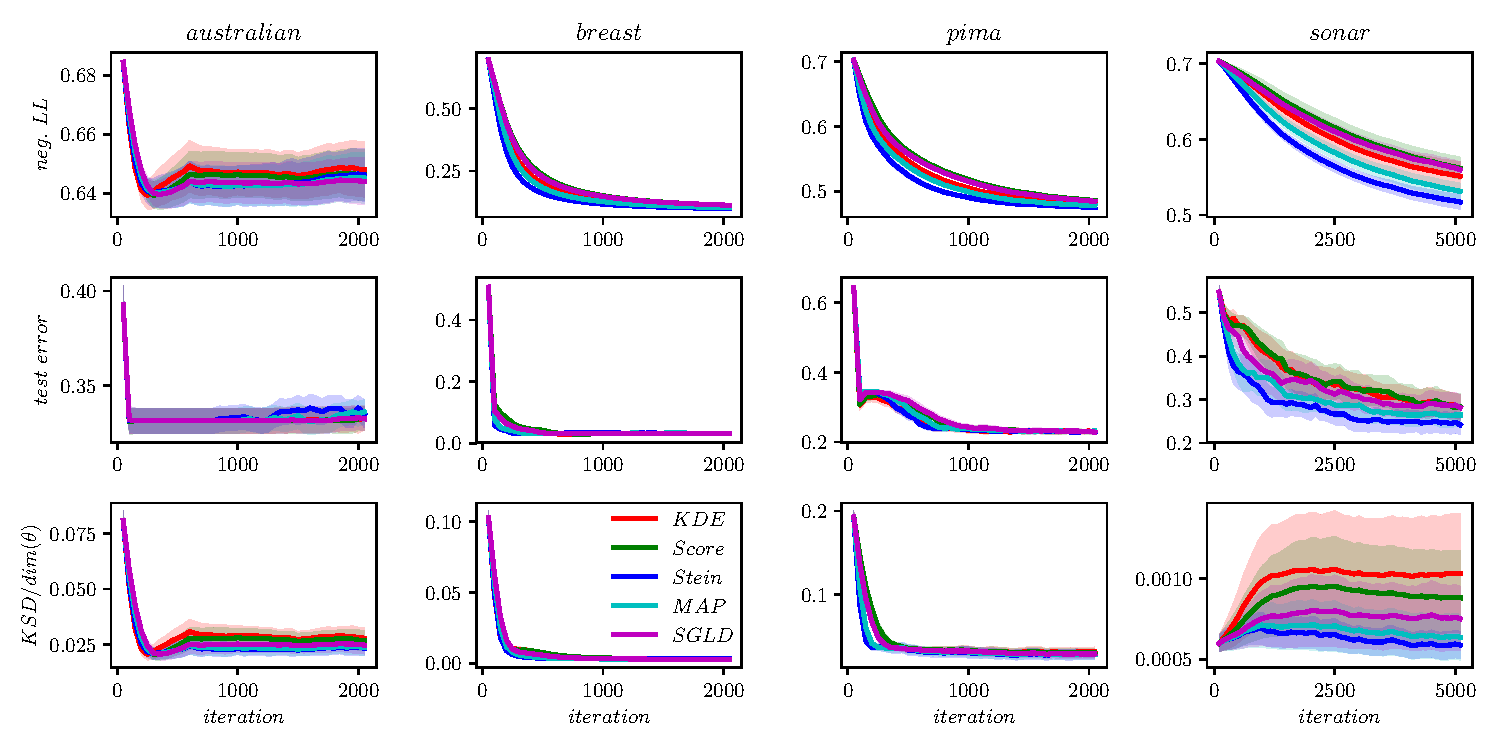
\includegraphics[width=1.0\linewidth]{figs/nn_sampler_results_new.pdf}
\vspace{-0.2in}
\caption{Generalisation performances for trained approximate posterior samplers.}
\vspace{-0.1in}
\label{fig:nn_sampler_results}
\end{figure}

Figure \ref{fig:nn_sampler_results} presents the (negative) test log-likelihood (LL), classification error, and an estimate of the KSD U-statistic $\mathcal{S}^2_U(p(\mparam | \D), q(\mparam))$ (with data sub-sampling) over 5 splits of each test dataset.\footnote{After conference publication (see publication page) I fixed a few issues of the previous implementation (mainly for the score matching estimator) and re-run the experiments, which is reported in this thesis.} 
%
The Stein approach performs equally well or a little better than SGLD in terms of test-LL and test error. The KDE method is slightly worse and is close to MAP, indicating that the KDE estimator does not provide a very informative gradient for the entropy term.
%
%The MAP model under-performs for test log-likelihood and KSD metrics, presumably because the noise variance $\bm{\sigma}$ has been turned off during learning thus having discovered an optimiser instead. 
%
The score matching estimator method produces the worst results among the trained samplers even after carefully tuning the bandwidth and the regularisation parameter $\eta$, although the difference is not significant. 
%
Future work should investigate the usage of advanced recurrent neural networks such as an LSTM \citep{hochreiter:lstm1997}, which is expected to return better performance.

\subsection{Towards addressing mode collapse in GANs using entropy regularisation}
GANs are notoriously difficult to train in practice. Besides the instability of gradient-based minimax optimisation which has been partially addressed by many recent proposals \citep{salimans:training2016, arjovsky:wgan2017, berthelot:began2017}, they also suffer from mode collapse. We propose adding an entropy regulariser to the GAN generator loss. Concretely, assume the generative model $p_{\mparam}(\x)$ is implicitly defined by $\x = \f_{\bm{\theta}}(\z), \z \sim p_0(\z)$, then the generator's loss is defined by 
\begin{equation}
\tilde{\mathcal{J}}_{\text{gen}}(\mparam) = \mathcal{J}_{\text{gen}}(\mparam) - \alpha \mathbb{H}[p_{\mparam}(\x)],
\label{eq:gan_regularised_general}
\end{equation}
where $\mathcal{J}_{\text{gen}}(\mparam)$ is the original loss function for the generator from any GAN algorithm and $\alpha$ is a hyper-parameter. In practice the gradient of (\ref{eq:gan_regularised_general}) is estimated using Monte Carlo.

As an illustrating example, in the following we consider the very recently proposed boundary equilibrium GAN (BEGAN) \citep{berthelot:began2017} approach. In BEGAN the discriminator is defined as an auto-encoder $D_{\hparam}(\x)$ that reconstructs the input $\x$. After selecting a ratio parameter $\gamma > 0$, a control rate $\beta_0$ initialised at 0, and a ``learning rate'' $\lambda > 0$ for the control rate, the loss functions for the generator $\x = \f_{\mparam}(\z), \z \sim p_0(\z)$ and the discriminator are:
\begin{equation}
\begin{aligned}
& \mathcal{J}(\x) =  || D_{\hparam}(\x) - \x ||, \quad || \cdot || = || \cdot ||_2^2 \text{ or } || \cdot ||_1, \\
& \mathcal{J}_{\text{gen}}(\mparam; \hparam) = \mathcal{J}(\f_{\mparam}(\z)), \quad \z \sim p_0(\z)  \\ 
& \mathcal{J}_{\text{dis}}(\hparam; \mparam) = \mathcal{J}(\x) - \beta_t \mathcal{J}_{\text{gen}}(\mparam; \hparam), \quad \x \sim \D \\
& \beta_{t+1} = \beta_t + \lambda (\gamma \mathcal{J}(\x) - \mathcal{J}(\f_{\mparam}(\z))).
\end{aligned}
\label{eq:began_original}
\end{equation}
The main idea behind BEGAN is that, as the reconstruction loss $\mathcal{J}(\cdot)$ is approximately Gaussian distributed, with $\gamma = 1$ the discriminator loss $\mathcal{J}_{\text{dis}}$ is (approximately) proportional to the Wasserstein distance between loss distributions induced by the data distribution $p_{\D}(\x)$ and the generator $p(\x)$. In practice it is beneficial to maintain the equilibrium $\gamma \mathbb{E}_{p_{\D}} \left[ \mathcal{J}(\x) \right] = \mathbb{E}_{p} \left[ \mathcal{J}(\x) \right] $ through the optimisation procedure described in (\ref{eq:began_original}) that is motivated by proportional control theory. This approach effectively stabilises training, however it suffers from catastrophic mode collapse problem (see the left most panel in Figure \ref{fig:gan_samples}). 

We empirically investigate the entropy regularisation idea on BEGAN using (continuous) MNIST. 
As described before, we simply subtract an entropy term from the generator's loss function, i.e. with $K$ samples $\z^1, ..., \z^k \sim p_0(\z)$,
\begin{equation}
\tilde{\mathcal{J}}_{\text{gen}}(\mparam; \hparam) = \frac{1}{K} \sum_{k=1}^K \mathcal{J}(\f_{\mparam}(\z^k)) + \alpha \frac{1}{K} \sum_{k=1}^K \log p(\f_{\mparam}(\z^k)),
\end{equation}
where the rest of the optimisation objectives remains as in (\ref{eq:began_original}). This procedure would maintain the equilibrium $\gamma \mathbb{E}_{p_{\D}} \left[ \mathcal{J}(\x) \right] = \mathbb{E}_{p} \left[ \mathcal{J}(\x) \right] - \alpha \mathbb{H}[p]$. We approximate the gradient $\nabla_{\mparam} \mathbb{H}[p]$ using the estimators presented above. For the purpose of updating the control rate $\beta_t$ two strategies are considered to approximate the contribution of the entropy term. The first proposal considers a plug-in estimate of the entropy term with a KDE estimate of $p(\x)$, which is consistent with the KDE estimator but not necessary with the other two (as they use kernels when representing $\log p(\x)$ or $\nabla_{\x} \log p(\x)$). The second one uses a proxy of the entropy loss $-\tilde{\mathbb{H}}[p] = \frac{1}{K} \sum_{k=1}^K \nabla_{\x^k} \log \hat{p}(\x^k)^{\text{T}} \x^k$ with $\nabla_{\x^k} \log \hat{p}(\x^k)$ is the approximate gradient obtained by the estimators. It is the surrogate loss used to (approximately) compute $\nabla_{\vparam} \mathbb{H}[p]$:
$$
\nabla_{\vparam} \mathbb{H}[p] \approx \nabla_{\vparam} \tilde{\mathbb{H}}[p] = \frac{1}{K} \sum_{k=1}^K \nabla_{\x^k} \log \hat{p}(\x^k)^{\text{T}} \nabla_{\vparam} \x^k.
$$

We compare the non-parametric V-statistic Stein gradient estimator to both KDE and score matching estimators. We use a convolutional generative network and a convolutional auto-encoder and select the hyper-parameters of BEGAN $\gamma \in \{0.3, 0.5, 0.7\}$, $\alpha \in [0, 1]$ and $\lambda = 0.001$. The Epanechnikov kernel $\mathcal{K}(\x, \x') := \frac{1}{d} \sum_{j=1}^d (1 - (x_j - x'_j)^2)$ is used as the pixel values lie in a unit interval (see Appendix \ref{sec:appendix_stein} for the expression of the score matching estimator), and to ensure the boundary condition we clip the pixel values into range $[10^{-8}, 1-10^{-8}]$. Readers are referred to Appendix \ref{sec:appendix_stein} for a detailed experimental set-up.

The generated images are visualised in Figure \ref{fig:gan_samples}. BEGAN without entropy regularisation fails to generate diverse samples even when trained with learning rate decay. The other three images clearly demonstrate the benefit of the entropy regularisation technique, with the Stein approach obtaining the highest diversity without compromising visual quality.

%
We further consider four metrics to assess the trained models quantitatively. First 500 samples are generated for each trained model, then we compute their nearest neighbours in the training set using $\ell_1$ distance, and obtain a probability vector $\mathbf{p}$ by averaging over these neighbour images' label vectors. In Figure \ref{fig:gan_results} we depict the entropy of $\mathbf{p}$  (top left), averaged $\ell_1$ distances to the nearest neighbour (top right), and the difference between the largest and smallest elements in $\mathbf{p}$ (bottom right). The error bars are obtained by 5 independent runs. These results demonstrate that the Stein approach performs significantly better than the other two, in that  it learns a better generative model not only faster but also in a more stable way. Interestingly the KDE approach achieves the lowest average $\ell_1$ distance to nearest neighbours, possibly because it tends to memorise training examples. We next train a fully connected network $\pi(\y|\x)$ on MNIST that achieves 98.16\% text accuracy, and compute on the generated images an empirical estimate of the inception score \citep{salimans:training2016} $\mathbb{E}_{p(\x)}[\mathrm{KL}[\pi(\y|\x) || \pi(\y)] ]$ with $\pi(\y) = \mathbb{E}_{p(\x)}[\pi(\y|\x)]$ (bottom left panel). High inception score indicates that the generate images tend to be both realistic looking and diverse, and again the Stein approach out-performs the others on this metric by a large margin. 

Concerning computation speed, all the three methods are of the same order: 10.20s/epoch for KDE, 10.85s/epoch for Score, and 10.30s/epoch for Stein.\footnote{All the methods are timed on a machine with an NVIDIA GeForce GTX TITAN X GPU.} This is because $K < d$ (in the experiments $K=100$ and $d=784$) so that the complexity terms are dominated by kernel computations ($\mathcal{O}(K^2 d)$) required by all the three methods. Also for a comparison, the original BEGAN method without entropy regularisation runs for 9.05s/epoch. Therefore the main computation cost is dominated by the optimisation of the discriminator/generator, and the proposed entropy regularisation can be applied to many GAN frameworks with little computational burden.

\begin{figure}[t]
\vspace{-0.2in}
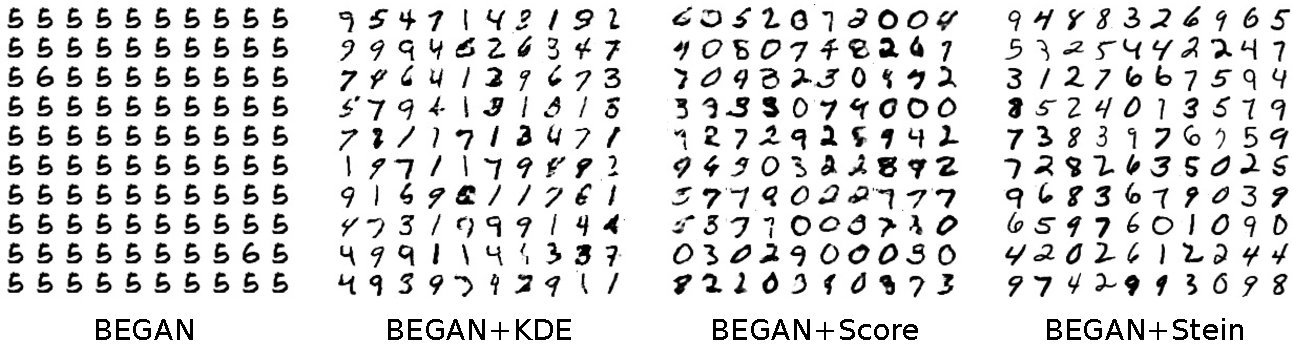
\includegraphics[width=1.0\linewidth]{figs/gan_samples.pdf}
\vspace{-0.2in}
\caption{Visualisation of generated images from trained BEGAN models.}
\label{fig:gan_samples}
\vspace{0.1in}
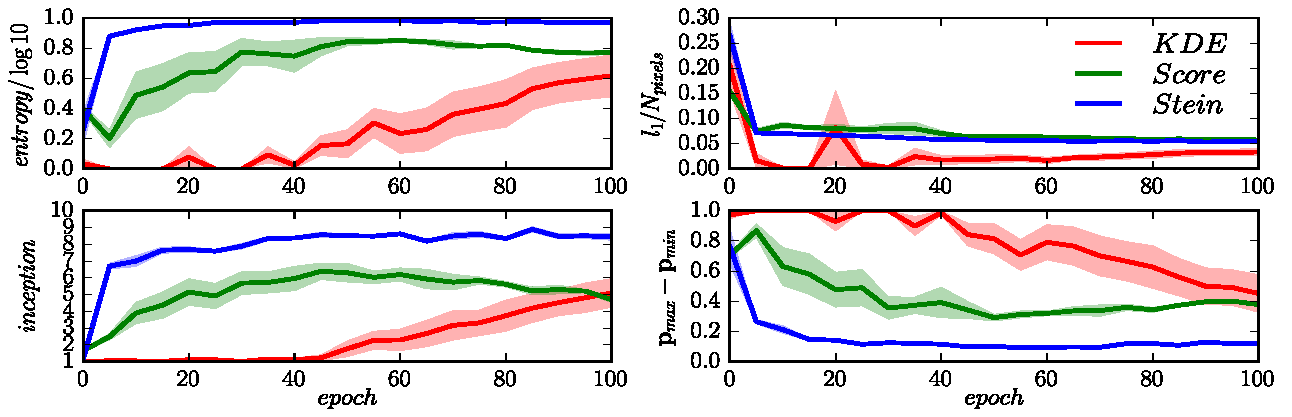
\includegraphics[width=1.0\linewidth]{figs/gan_results.pdf}
\vspace{-0.2in}
\caption{Quantitative evaluation on entropy regularised BEGAN. The higher the better for the LHS panels and the other way around for the RHS ones. See main text for details.}
\vspace{-0.1in}
\label{fig:gan_results}
\end{figure}

\section{Summary}
\label{sec:conclusions}

We have presented the Stein gradient estimator as a novel generalisation to the score matching gradient estimator. With a focus on learning implicit models, we have empirically demonstrated the efficacy of the proposed estimator by showing state-of-the-art results on three canonical learning tasks: approximating gradient-free MCMC, meta-learning for approximate posterior samplers, and unsupervised learning for image generation. Future work will expand the understanding of gradient estimators in both theoretical and practical sides. Theoretical development will compare both the V-statistic and U-statistic Stein gradient estimators. Practical work will improve the sample efficiency of kernel estimators in high dimensions and develop fast yet accurate approximations to the matrix inversion part. Finally follow-up work will study the generalisation of the Stein gradient estimator to non-kernel settings and discrete distributions.


\vspace{3em}
{\Large
\noindent \hrulefill \hspace{0.2cm} \raisebox{-4pt}[10pt][10pt]{\decofourleft ~  \decosix ~ \decofourright} \hspace{0.1cm} \hrulefill
\vspace{2em}
}

Here comes the end of the second theme of the thesis, where we have discussed principles of approximate inference algorithm design (Chapter \ref{chap:wild}) and presented one concrete example (Chapter \ref{chap:grad_approx}) on learning wild approximations. Readers might have noticed that wild approximate inference is still a very new research direction: many related papers in citation are freshly baked within a year of this thesis submission, and the proposals in development are inspired by recent success in machine learning and deep learning. Thus both theoretical analyses and extensive comparisons to traditional approaches are much in need, which will then help identify the ideal application scenarios and possibly potential pitfalls of the method.

The presented two themes have substantial differences. In the next chapter, which concludes the thesis, I will summarise the contributions of the thesis to the approximate inference community, and discuss the connections and comparisons between the two themes. Expositions of important research questions will also be provided, and hopefully this will serve as a principled guide for future development of approximate inference algorithms.